% a-project.tex, v-1.0.3 marcoreis baseado no
% abntex2-modelo-trabalho-academico.tex, v-1.9.7 laurocesar
% Copyright 2012-2018 by abnTeX2 group at http://www.abntex.net.br/ 
% 
% This work consists of the files ........
% 
% -----------------------------------------------------------------------------
% Modelo para desenvolvimento de documentação de projetos acadêmicos
% (tese de doutorado, dissertação de mestrado e trabalhos de monografias em geral) 
% em conformidade com ABNT NBR 14724:2011: Informação e documentação. 
% -----------------------------------------------------------------------------
% Opções para a documentação
%
% Fancy page headings 
%\documentclass[fancyheadings, subook]{Classes/a-prj}
%\documentclass[fancyheadings, sureport]{Classes/a-prj}
%
% Fancy chapters and sections headings 
%\documentclass[fancychapter, subook]{Classes/a-prj}
%\documentclass[fancychapter, sureport]{Classes/a-prj}
%
% Fancy page , chapters and sections headings
%\documentclass[fancyheadings, fancychapter, subook]{Classes/a-prj}
\documentclass[fancyheadings, fancychapter, sureport]{Classes/a-prj}
%
% -----------------------------------------------------------------------------
% Alguns comandos para a fancy page headings)
%
% Page header line width
%\footlinewidth{value}
%
% Page footer line width
%\headlinewidth{value}
%
% Page header and footer line width
%\headingslinewidth{value}
%
% Page header and footer lines without text
%\headingslinesonly
%
% The default line width is 0.3pt.
% Set the value to 0pt to remove the page header and/or footer line
%
% -------------------------------------------------------------------------------
% Formato de figuras suportado
% -------------------------------------------------------------------------------
% O formato das figuras depende da forma como o arquivo de saída é gerado.
% As figuras inseridas na pasta Figures serão automaticamente reconhecidas sem
% a necessidade de inserir a extensão do arquivo.
%
% O pdfLaTEX (PDF) suporta figuras com as extensões: pdf, jpg, png e mps.
%
% -------------------------------------------------------------------------------
% Árvore do diretório a-project.tex
%  Diretório
%       \Classes        (requerido)
%       \Figures        (requerido) --------------------------------->
%       \Figures\PDF    (optional)
%       \Figures\JPG    (optional) Figures located within these
%       \Figures\PNG    (optional) folders are searched automatically
%       \Figures\MPS    (optional)  by the a-prj class.
%       \Figures\EPS    (optional)
%       \Figures\PS     (optional) <--------------------------------
%       \Tables         (requerido)
%       \Others         (requerido)
%       \Chapters       (requerido)
%       \Appendices     (optional)
%       \References     (requerido)
%
% -------------------------------------------------------------------------------
% PDF File resumo
\ifpdf
    \hypersetup{
    	backref,
        colorlinks  = true,
        pdftitle    = Modelo de documentação,
        pdfauthor   = {Marco Reis, marco.a.reis@gmail.com},
        pdfsubject  = Mestre em Engenharia,
        pdfcreator  = Subtitulo,
        pdfproducer = PDFLatex,
        pdfkeywords = {documentação, latex, dissertação, tese}}
 \fi
%
% -------------------------------------------------------------------------------
% Relação de pacotes opcionais utilizados
\usepackage[utf8]{inputenc}
\usepackage[brazil]{babel}
\usepackage{longtable}
\usepackage{dcolumn}
\usepackage{multirow}
\usepackage{lscape}
%\usepackage{graphicx}
\usepackage{rotating}
%\usepackage{float,subfigure}
%\usepackage{graphicx, subfigure}
\usepackage{cite}
\usepackage[left=3cm,top=3cm,right=2cm,bottom=2cm]{geometry}
\usepackage[alf]{abntex2cite}
\usepackage{ifpdf}
\usepackage{shadow}
\usepackage{wrapfig}
\usepackage[normalem]{ulem}
\usepackage{makeidx}
\usepackage{yfonts}
\usepackage{algorithm}
\usepackage{algorithmic}
\usepackage{lmodern}
\usepackage[T1]{fontenc}
\usepackage{indentfirst}
\usepackage{color}
\usepackage{microtype}
\usepackage{lipsum}
\usepackage{caption}
\usepackage{subcaption}
%
\makeindex 
\setlength{\LTcapwidth}{\textwidth}
%
\newtheorem{theorem}{Teorema}
\newtheorem{definition}[theorem]{Definição}
%
% -------------------------------------------------------------------------------
% Configurações do pacote backref
\renewcommand{\backrefpagesname}{Citado na(s) página(s):~}
% Texto padrão antes do número das páginas
\renewcommand{\backref}{}
% Define os textos da citação
\renewcommand*{\backrefalt}[4]{
	\ifcase #1 %
		Nenhuma citação no texto.%
	\or
		Citado na página #2.%
	\else
		Citado #1 vezes nas páginas #2.%
	\fi
}
% 
% -------------------------------------------------------------------------------
% Início do documento raiz
\begin{document}
% Definição do título da página
    \university{Centro Universitário SENAI CIMATEC}
	%\faculty{Programa de...}
	%\school{Escola de...}
% 
    %\course{Engenharia Elétrica}
    \typework{Centro de Competência em Robótica e Sistemas Autônomos}
% 
	%\course{Mestrado em Modelagem Computacional e Tecnologia Industrial}
	%\typework{Disserta\c{c}\~ao de mestrado}
	%\typework{Exame de Qualificação de Mestrado}
% 
	%\course{Engenharia Elétrica}
	%\typework{Tese de doutorado}
	%\typework{Exame de Qualificação de doutorado}
%
% -------------------------------------------------------------------------------
% Informações gerais
    \thesistitle{Relatório final do projeto ``Novos Telentos''}
    \hidevolume
    \thesisvolume{Volume 1 of 1}
    \thesisauthor{Vinicius José Gomes de Araújo Felismino}
    \thesisauthorr{John Nash}
    \thesisauthorrr{James Clerk Maxwell}
    \thesisauthorrrr{Nikola Tesla}
    \thesisauthorrrrr{Sir Isaac Newton}
    %\thesisadvisor{Prof. Marco Reis, M.Eng.}
    %\hidecoadvisor
    %\thesiscoadvisor{Marco Reis}
    \thesisdegreetitle{Bacharel em Engenharia}
    \thesismonthyear{Agosto de 2020}
% 
    \maketitlepage
%
% ----------------------------------------------------------------------------
% Inserir Folha de rosto, Nota de estilo, folha de assinaturas, dedicatoria
    \begin{folharosto}

\begin{center}
\theauthor \\
\theauthorr \\
\theauthorrr \\
\theauthorrrr \\
\theauthorrrrr \\
\end{center}
\ \\
\ \\
\ \\
\ \\
\ \\
\begin{spacing}{2}
   \begin{center}
   {\LARGE {\bf \thetitle}}
   \end{center}
\end{spacing}
\ \\
\ \\
\ \\
\vspace*{85mm}
% \begin{flushright}

%    \begin{list}{}{
%       \setlength{\leftmargin}{7.5cm}
%       \setlength{\rightmargin}{0cm}
%       \setlength{\labelwidth}{0pt}
%       \setlength{\labelsep}{\leftmargin}}

%       \item \thetypework apresentada ao \thefaculty, Curso de \thecourse
%       do \theuniversity, como requisito parcial para a obten\c{c}\~ao do
%       t\'itulo de {\bf \thedegreetitle}.

%       \begin{list}{}{
%       \setlength{\leftmargin}{0cm}
%       \setlength{\rightmargin}{0cm}
%       \setlength{\labelwidth}{0pt}
%       \setlength{\labelsep}{\leftmargin}}

%       \item \'Area de conhecimento: Interdisciplinar

%       \item Orientador: \theadvisor
%       \newline \hspace*{2.1cm}  %{\it \theuniversity}

%       \end{list}
%    \end{list}

% \end{flushright}
\ \\
\ \\
\ \\
\ \\
%\begin{spacing}{1.5}
   \begin{center}
   Salvador \par
   \theuniversity \par
   2020
   \end{center}
%\end{spacing}

\end{folharosto}

    %\begin{notaestilo}
Esta \thetypeworkthree foi elaborada considerando as normas de
estilo (i.e. est\'eticas e estruturais) propostas aprovadas pelo
colegiado do \thefacultytwo e est\~ao dispon\'iveis em formato
eletr\^onico ({\it download} na P\'agina Web
http:$//$ead.fieb.org.br$/$portal\_faculdades$/$dissertacoes-e-teses-mcti.html
ou solicita\c{c}\~ao via e-mail \`a secretaria do
programa) e em formato impresso somente para consulta. \\

Ressalta-se que o formato proposto considera diversos itens das
normas da Associa\c{c}\~ao Brasileira de Normas T\'ecnicas (ABNT),
entretanto opta-se, em alguns aspectos, seguir um estilo pr\'oprio
elaborado e amadurecido pelos professores do programa de
p\'os-gradua\c{c}\~ao supracitado.

\end{notaestilo}

    %\begin{folhaassinaturas}

%\thispagestyle{empty}

\def\signature#1#2{\parbox[b]{1in}{\smash{#1}\vskip12pt}
\hfill \parbox[t]{3in}{\shortstack{\vrule width 3in height
0.4pt\\\small#2}}}

\def\InstituicaoMembro#1#2{\parbox[b]{1in}{\smash{#1}\vskip12pt}
\hfill \parbox[t]{3in}{\shortstack{\vrule width 3in \\\small#2}}}

\def\signaturepage{%

    \begin{spacing}{1.5}
        \begin{center}
        {\LARGE \theuniversity} \\
        {\large \thefaculty} \\
        {\large \thecourse} \\
        \end{center}
    \end{spacing}

   \vskip 0.25in plus 0.4in minus 0.1in

    \begin{spacing}{1.5}
        \begin{sloppypar}
        A Banca Examinadora, constitu\'ida pelos professores abaixo
        listados, leram e recomendam a aprova\c{c}\~ao [com distin\c{c}\~ao] da
        \thetypeworktwo, intitulada ``\thetitle",
        apresentada no dia (dia) de (m\^es) de (ano), como requisito
        parcial para a obten\c{c}\~ao do t\'itulo de {\bf \thedegreetitle}.\\
        \end{sloppypar}
    \end{spacing}

    \def\sigskip{\vskip0.15in plus 0.2in minus 0.1in}
    \def\beginskip{\vskip0.3875in plus 0.2in minus 0.1in}

    \beginskip
    \signature{Orientador:}{Prof. Dr. \theadvisor} \\
    \InstituicaoMembro{}{\theuniversity} \\

    \sigskip
    \beginskip
    \signature{Membro externo da Banca:}{Prof. Dr. Nome completo} \\
    \InstituicaoMembro{}{Institui\c{c}\~ao do membro da banca} \\

    \sigskip
    \beginskip
    \signature{Membro externo da Banca:}{Prof. Dr. Nome completo} \\
    \InstituicaoMembro{}{Institui\c{c}\~ao do membro da banca} \\

    %\sigskip
    %\beginskip
   % \signature{Membro interno da Banca:}{Prof. Dr. Nome completo} \\
   % \InstituicaoMembro{}{Institui��o do membro da banca} \\

    \vfill
    \newpage
    \setcounter{page}{3}
}
%*********************************************************************


\signaturepage


\end{folhaassinaturas}

    %\include{Others/dedicatoria}
    %\include{Others/agradecimentos}
%
% ----------------------------------------------------------------------------
% Resumo/abstract, sumário e siglas
    \begin{romanpagenumbers}
        \begin{thesisresumo}
Escreva aqui o resumo da disserta\c{c}\~ao, incluindo os contextos geral e espec\'ifico, dentro dos quais a pesquisa foi realizada, o objetivo da pesquisa, assun\c{c}\~ao filos\'ofica, os m\'etodos de pesquisa usados e as poss\'iveis contribui\c{c}\~oes que o que \'e proposto pode trazer \`a sociedade.

\ \\

% use de três a cinco palavras-chave

\textbf{Palavras-chave}: Palavra-chave 1, Palavra-chave 2, Palavra-chave 3, Palavra-chave 4, Palavra-chave 5

\end{thesisresumo}

        \begin{thesisabastract}
Escreva aqui, em ingl\^es, o resumo da disserta\c{c}\~ao, incluindo os contextos geral e espec\'ifico, dentro dos quais a pesquisa foi realizada, o objetivo da pesquisa, assun\c{c}\~ao filos\'ofica, os m\'etodos de pesquisa usados e as poss\'iveis contribui\c{c}\~oes que o que \'e proposto pode trazer \`a sociedade. 

\ \\

% use de tr�s a cinco palavras-chave

\textbf{Keywords}: Keyword 1, Keyword 2, Keyword 3, Keyword 4, Keyword 5

\end{thesisabastract}

        % Make list of contents, tables and figures
        \thesiscontents
        %Include other required section
        %\begin{thesisabbreviations}
\begin{footnotesize}
\begin{longtable}[l]{p{2cm}l}
  tprax   \dotfill & \thefaculty \\
  WWW       \dotfill &  World Wide Web \\
\end{longtable}
\end{footnotesize}
\end{thesisabbreviations}

        %\begin{thesissymbols}
\begin{footnotesize}
\begin{longtable}[l]{p{2cm}l}
  $\partial$   \dotfill  & Bla bla bla \\
  $\prod$       \dotfill & ble ble ble \\
  $\partial$   \dotfill  & Bla bla bla \\
  $\prod$       \dotfill & ble ble ble \\
  $\partial$   \dotfill  & Bla bla bla \\
  $\prod$       \dotfill & ble ble ble \\
  $\partial$   \dotfill  & Bla bla bla \\
  $\prod$       \dotfill & ble ble ble \\
  $\partial$   \dotfill  & Bla bla bla \\
  $\prod$       \dotfill & ble ble ble \\
  $\partial$   \dotfill  & Bla bla bla \\
  $\prod$       \dotfill & ble ble ble \\
  $\partial$   \dotfill  & Bla bla bla \\
  $\prod$       \dotfill & ble ble ble \\
  $\partial$   \dotfill  & Bla bla bla \\
  $\prod$       \dotfill & ble ble ble \\
  $\partial$   \dotfill  & Bla bla bla \\
  $\prod$       \dotfill & ble ble ble \\
  $\partial$   \dotfill  & Bla bla bla \\
  $\prod$       \dotfill & ble ble ble \\
  $\partial$   \dotfill  & Bla bla bla \\
  $\prod$       \dotfill & ble ble ble \\
  $\partial$   \dotfill  & Bla bla bla \\
  $\prod$       \dotfill & ble ble ble \\
  $\partial$   \dotfill  & Bla bla bla \\
  $\prod$       \dotfill & ble ble ble \\
  $\partial$   \dotfill  & Bla bla bla \\
  $\prod$       \dotfill & ble ble ble \\
  $\partial$   \dotfill  & Bla bla bla \\
  $\prod$       \dotfill & ble ble ble \\
  $\partial$   \dotfill  & Bla bla bla \\
  $\prod$       \dotfill & ble ble ble \\
  $\partial$   \dotfill  & Bla bla bla \\
  $\prod$       \dotfill & ble ble ble \\
  $\partial$   \dotfill  & Bla bla bla \\
  $\prod$       \dotfill & ble ble ble \\
  $\partial$   \dotfill  & Bla bla bla \\
  $\prod$       \dotfill & ble ble ble \\          
\end{longtable}
\end{footnotesize}
\end{thesissymbols}

        %Switch the page numbering back to the default format
    \end{romanpagenumbers}
%
% ---------------------------------------------------------------------------
% Include thesis chapters
    \parskip=\baselineskip
    \chapter{Introdução}
\label{chap:intro}

O presente documento visa agrupar todos os conteúdos abordados e mostrar os resultados das atividades de pesquisa, criação e seleção de soluções para todos os desafios propostos pelos os orientadores e pesquisadores do Centro de Competência em Robótica e Sistemas Autônomos (CCRoSA) do SENAI-CIMATEC. Todas estas atividades ocorram durante o processo do curso de formação em robótica e sistemas autônomos, oferecido pela instituição, que teve inicio no dia 9 de novembro de 2019 e um prazo de duração de 1 ano.



%--------- NEW SECTION ----------------------
\section{Objetivos}
\label{sec:obj}

O objetivo geral deste relatório é relatar como o curso foi estruturado, ou seja, será apresentado todas as atividades e conhecimentos adiquiridos durante todo o periodo de duração da formação. 


\subsection{Objetivos Específicos}
\label{ssec:objesp}

O objetivo específico deste documento é agrupar todas as soluções para os diversos desafios proposto. 

%--------- NEW SECTION ----------------------
\section{Justificativa}
\label{sec:justi}

Com os crecentes avanços técnológicos, principalmente na área da robótica, a instituição SENAI-CIMATEC observou que era necessário mão de obra qualificada neste campo. Partindo desta premissa e adotando-a como seu principal objetivo lançou o programa de formação ``Novos Talentos - Robótica e Sistemas Autônomos'' para buscar o aumento da oferta de pessoal qualificado, em especial para as competências de robótica e sistemas Autônomos. 


%--------- NEW SECTION ----------------------
\section{Organização do documento}
\label{section:organizacao}

Este documento apresenta $4$ capítulos e está estruturado da seguinte forma:

\begin{itemize}

  \item \textbf{Capítulo \ref{chap:intro} - Introdução}: Contextualiza o âmbito, no qual o programa proposto está inserido. Apresenta, portanto, os objetivos, justificativa e como este programa foi estruturado;
  % \item \textbf{Capítulo \ref{chap:fundteor} - Fundamentação Teórica}: XXX;
  \item \textbf{Capítulo \ref{chap:mat} - Desenvolvimento}: Contextualiza cada problema proposto pelos os orientadores e pesquisadores do CCRoSA. Além disso, será demonstrado os materiais e métodos utilizados para a solução dos mesmos;
  \item \textbf{Capítulo \ref{chap:result} - Resultados}: Será exibido os principais resultados obtidos com a resolução de cada desafio proposto;
  \item \textbf{Capítulo \ref{chap:conc} - Conclusão}: Apresenta a conclusão geral do programa além de apresentar uma conclusão específica para cada desafio.

\end{itemize}

    \chapter{Fundamentação Teórica}
\label{chap:fundteor}

\begin{flushright}

   \begin{list}{}{
      \setlength{\leftmargin}{4.5cm}
      \setlength{\rightmargin}{0cm}
      \setlength{\labelwidth}{0pt}
      \setlength{\labelsep}{\leftmargin}}
      \item Quanto maior for a rapidez de transformação de uma
      sociedade, mais temporárias são as necessidades
      individuais. Essas flutuaçõess tornam ainda mais acelerado
      o senso de turbilh da sociedade.

      \begin{list}{}{
      \setlength{\leftmargin}{0cm}
      \setlength{\rightmargin}{0cm}
      \setlength{\labelwidth}{0pt}
      \setlength{\labelsep}{\leftmargin}}
      \item (Alvin Toffler)
      \end{list}
   \end{list}
\end{flushright}

\begin{flushright}
  Quanto maior for a rapidez de transformação de uma \\
  sociedade, mais temporárias são as necessidades \\
  individuais. Essas flutuações tornam ainda mais \\
  acelerado o senso de turbilhão da sociedade. \\
  \ \\
  (Alvin Toffler)
\end{flushright}

%--------- NEW SECTION ----------------------
\section{Estudo do estado da arte}
\label{sec:sota}
\lipsum[1]

%---------------picture------------------------------------
\begin{figure} [h!]												 
	\centering													 
	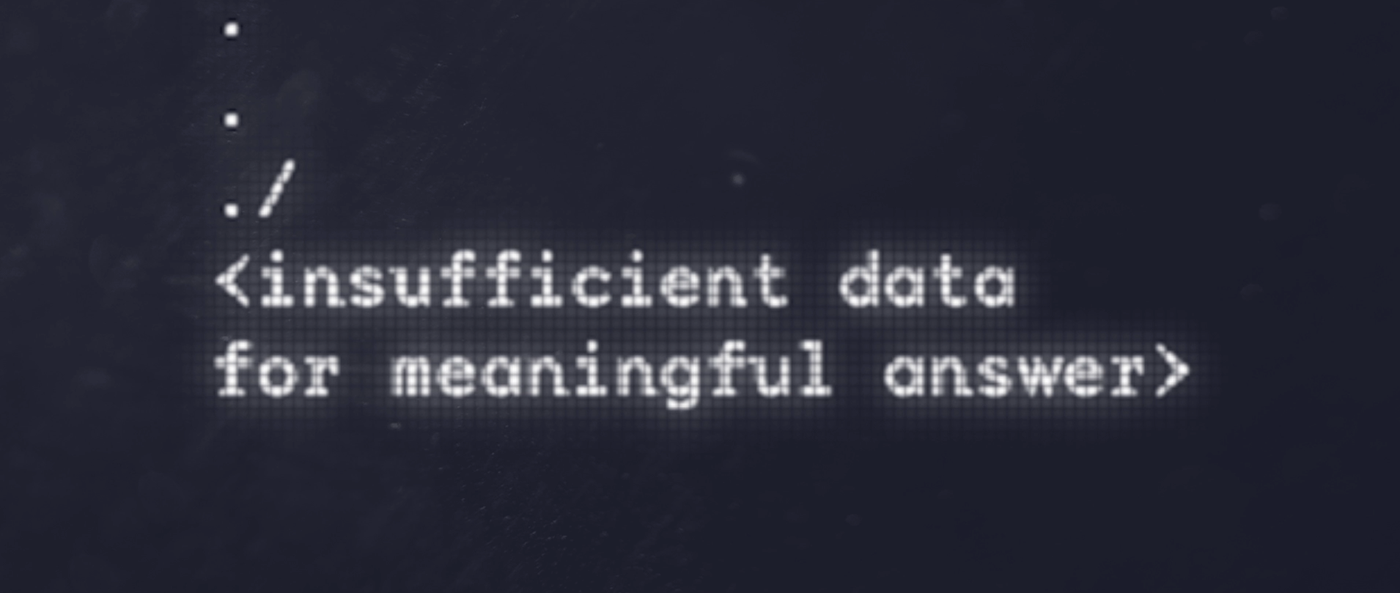
\includegraphics[width=0.6\textwidth]{./lq}				 
	\caption{Insufficient data.}		
	\label{img:ihuma}												 
\end{figure}													 
%----------------------------------------------------------

%--------- NEW SECTION ----------------------
\section{Assunto 1}
\label{sec:ass1}
\lipsum[1]



%---------------picture------------------------------------
% \begin{figure}
%     \centering
%     \subfigure[Figure A]{\label{fig:a}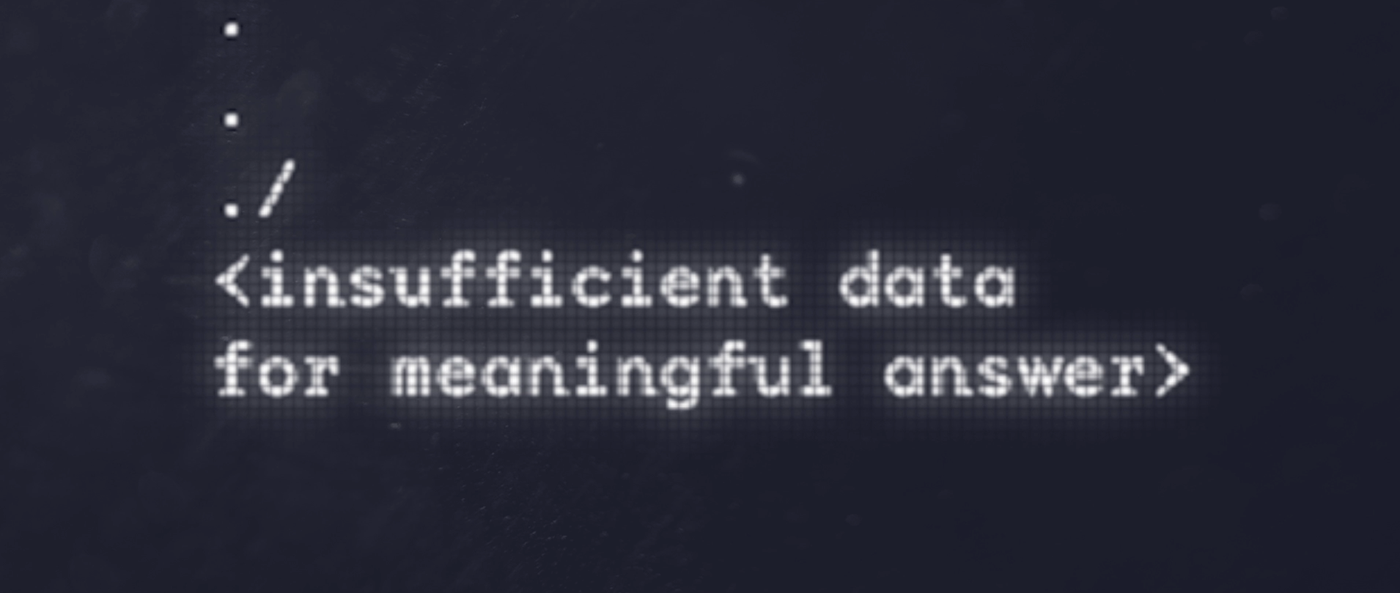
\includegraphics[width=60mm]{./lq}}
%     \subfigure[Figure B]{\label{fig:b}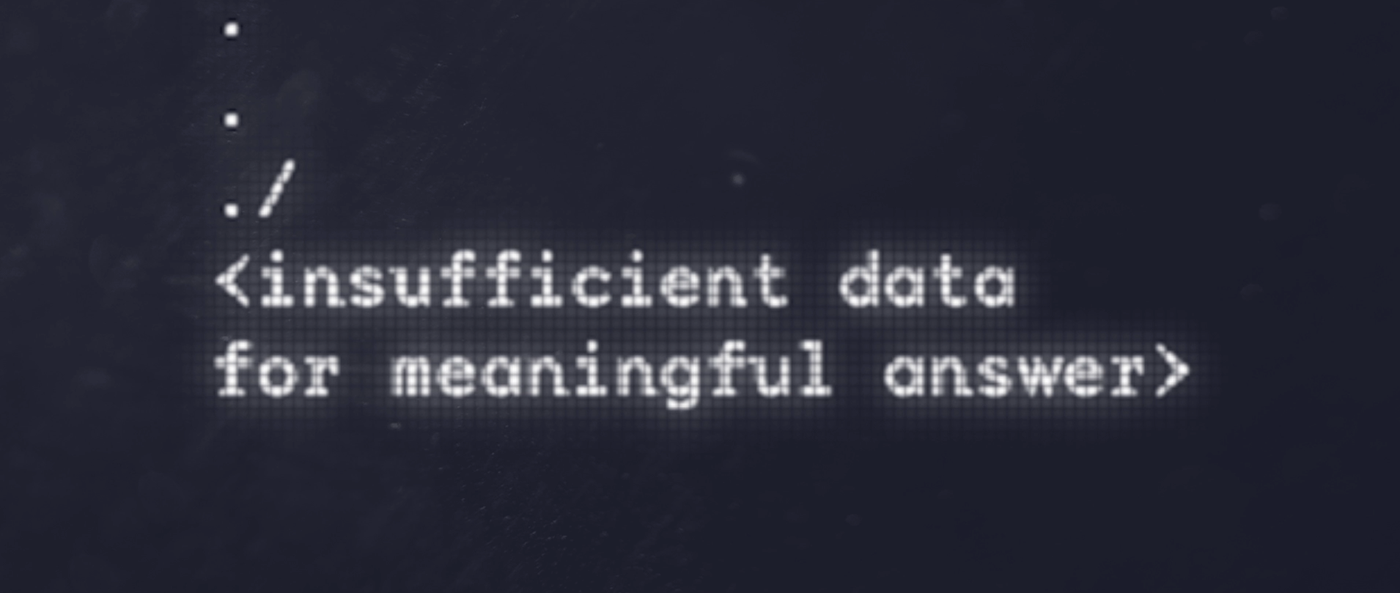
\includegraphics[width=60mm]{./lq}}
%     \subfigure[Figure C]{\label{fig:c}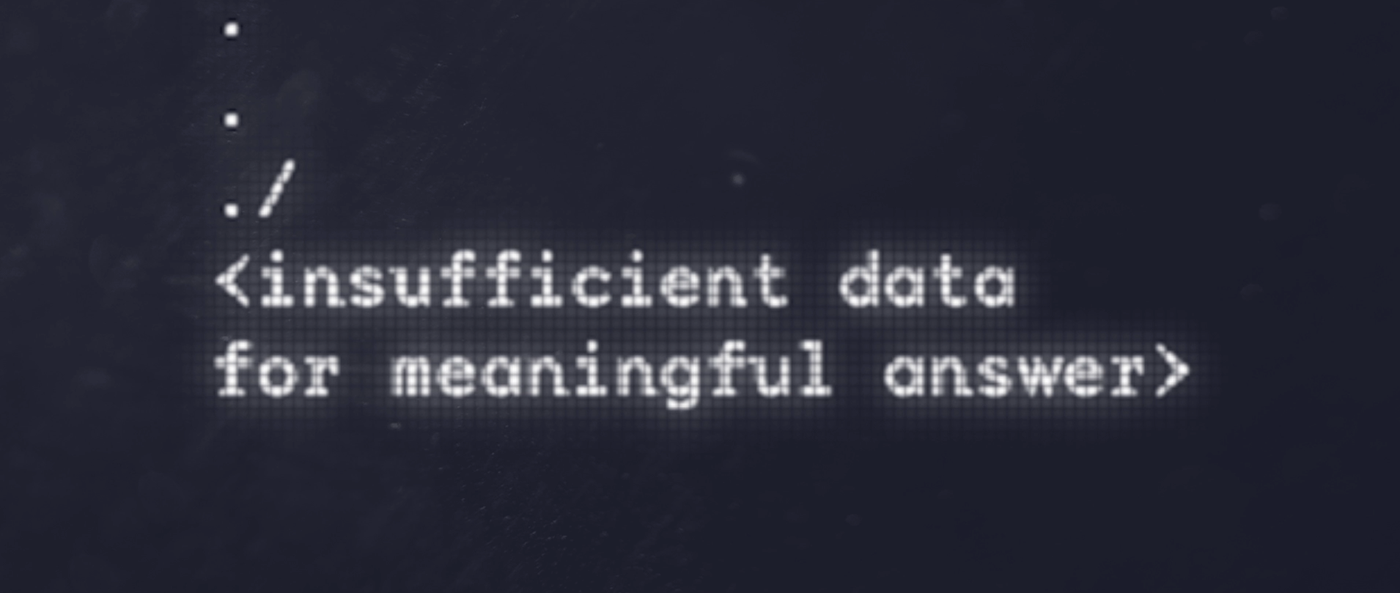
\includegraphics[width=\textwidth]{./lq}}
%     \caption{Three simple graphs}
%     \label{fig:three graphs}
% \end{figure}
%----------------------------------------------------------

\begin{figure}
    \centering
    \begin{subfigure}[b]{0.3\textwidth}
        \centering
        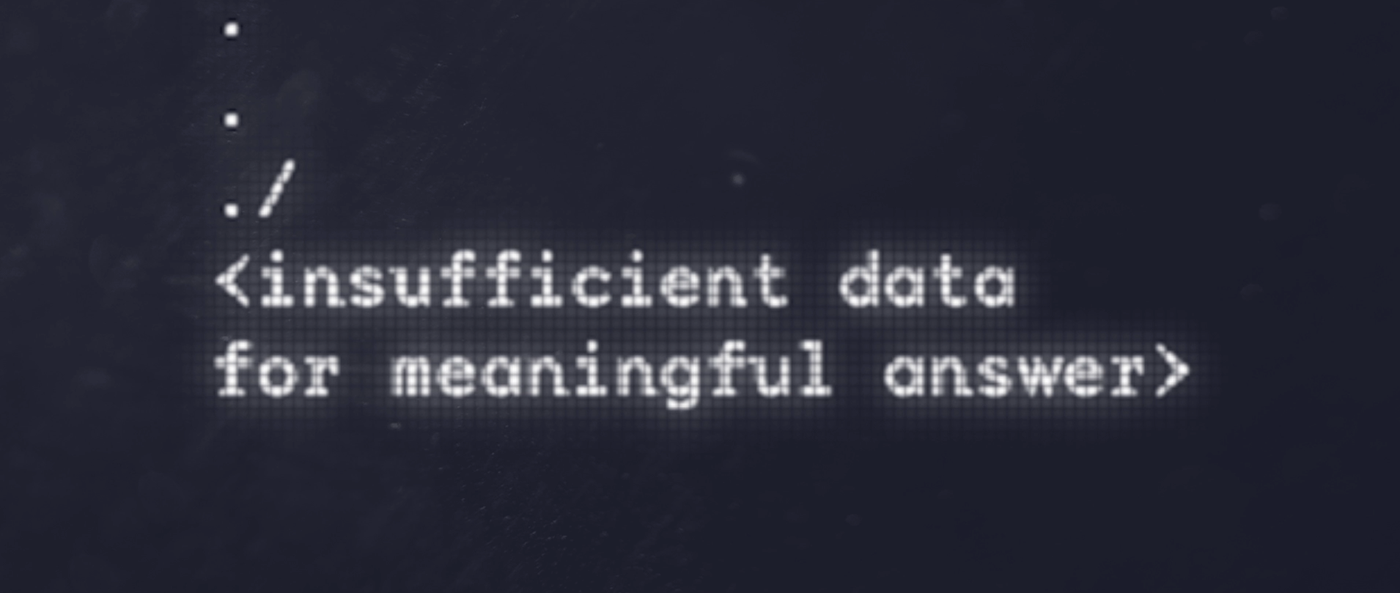
\includegraphics[width=\textwidth]{./lq}
        \caption{$y=x$}
        \label{fig:y equals x}
    \end{subfigure}
    \hfill
    \begin{subfigure}[b]{0.3\textwidth}
        \centering
        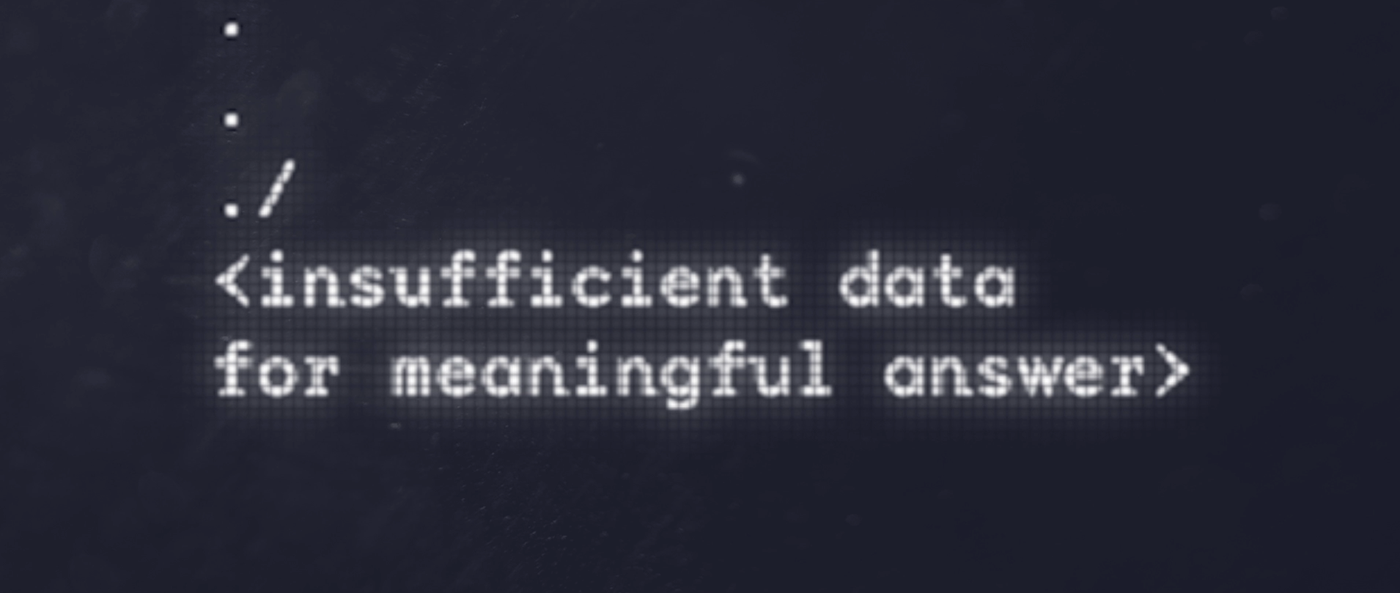
\includegraphics[width=\textwidth]{./lq}
        \caption{$y=3sinx$}
        \label{fig:three sin x}
    \end{subfigure}
    \hfill
    \begin{subfigure}[b]{0.3\textwidth}
        \centering
        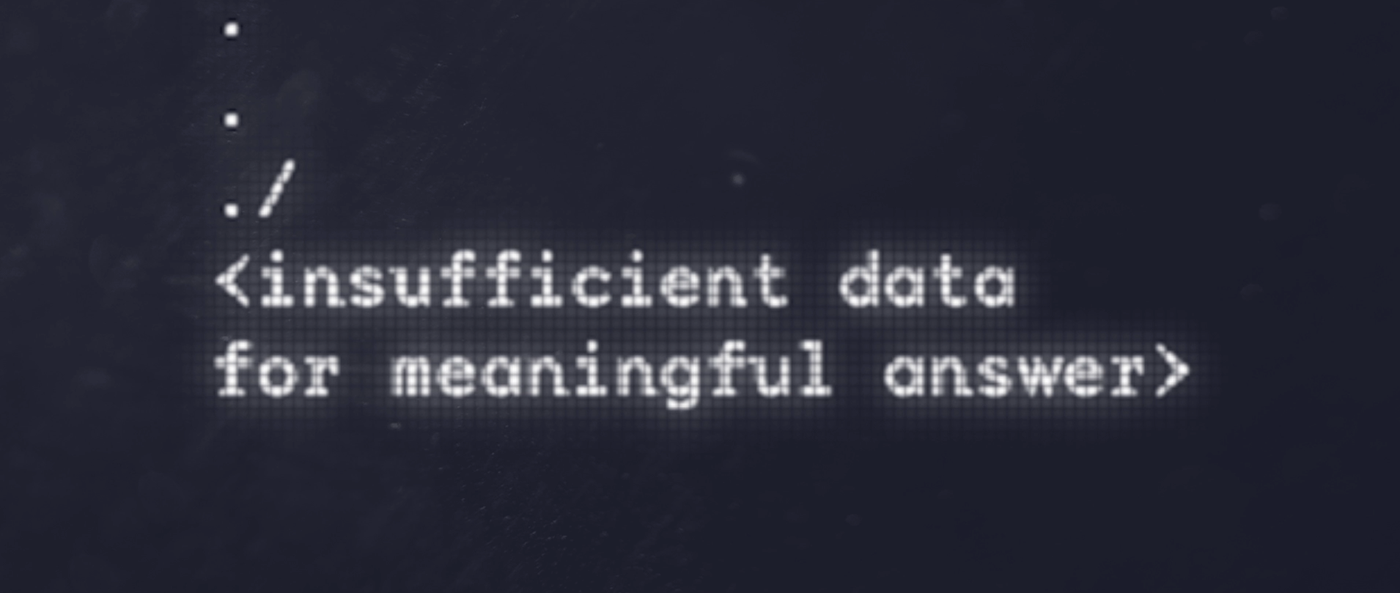
\includegraphics[width=\textwidth]{./lq}
        \caption{$y=5/x$}
        \label{fig:five over x}
    \end{subfigure}
       \caption{Three simple graphs}
       \label{fig:three graphs}
\end{figure}


%--------- NEW SECTION ----------------------
\section{Assunto 2}
\label{sec:ass2}
flkjasdlkfjasdlkfjs

\begin{table}[h]
    \begin{subtable}[h]{0.45\textwidth}
        \centering
        \begin{tabular}{l | l | l}
        Day & Max Temp & Min Temp \\
        \hline \hline
        Mon & 20 & 13\\
        Tue & 22 & 14\\
        Wed & 23 & 12\\
        Thurs & 25 & 13\\
        Fri & 18 & 7\\
        Sat & 15 & 13\\
        Sun & 20 & 13
       \end{tabular}
       \caption{First Week}
       \label{tab:week1}
    \end{subtable}
    \hfill
    \begin{subtable}[h]{0.45\textwidth}
        \centering
        \begin{tabular}{l | l | l}
        Day & Max Temp & Min Temp \\
        \hline \hline
        Mon & 17 & 11\\
        Tue & 16 & 10\\
        Wed & 14 & 8\\
        Thurs & 12 & 5\\
        Fri & 15 & 7\\
        Sat & 16 & 12\\
        Sun & 15 & 9
        \end{tabular}
        \caption{Second Week}
        \label{tab:week2}
     \end{subtable}
     \caption{Max and min temps recorded in the first two weeks of July}
     \label{tab:temps}
\end{table}
    \chapter{Desenvolvimento}
\label{chap:mat}

Neste capítulo será descrito cada desafio proposto pelos os orientadores e pesquisadores do CCRoSA durante o ano letivo e os materiais e métodos adotados para a concepção das soluções para cada um deles.

\section{Desafio 1.0 - Busca e navegação autônoma com o Husky.}

Este desafio teve como objetivo de realizar a simulação de uma determinada missão. Esta consistiu em realizar a navegação autônoma, no pátio do CIMATEC 4, com o \textit{Husky} da \textit{Clearpath Robotics} a fim de procurar e identificar uma bola amarela posta no mapa. Para concepção da solução foi utilizado o \textit{Robot Operating System (ROS)}, o \textit{software Gazebo} com auxilio da ferramenta de visualização \textit{Rviz}. O repositório com a solução pode ser encontrado no link \url{https://github.com/ViniciusFelismino8/desafio}.

\section{Desafio 2.0 - Concepção de um manipulador robótico.}
\label{sec:desafio2.0}

A princípio o objetivo deste desafio foi construir um manipulador robótico e através da identificação de marcadores visuais realizar a tarefa de acionamento de um painel elétrico. Devido aos efeitos da COVID-19, as atividades presenciais no laboratório tiveram que ser suspensas, com isso, afetou diretamente na construção física do manipulador. Portanto, a solução entregue para este desafio foi realizada apenas em ambiente simulado. 

Para concepção da solução foi formado um grupo que, além de mim, detinha mais três bolsistas do programa, entre eles, Jéssica Motta, Leonardo Mendes e Miguel Felipe. A modelagem 3D da estrutura física do manipulador foi feita no \textit{software OnShape}, o \textit{framework} de robótica e manipulação utilizado foi o \textit{ROS} e \textit{MoveIt}, respectivamente. Por fim, a simulação da tarefa foi realizada no \textit{software Gazebo} com auxilio da ferramenta de visualização \textit{Rviz}. O relatório final deste projeto pode ser visto no Apêndice \ref{appen:timon_hm_parcial}.

\section{Desafio 2.5 - Simular a marcha e corrida de revezamento com o Darwin-OP}
\label{sec:desafio2.5}

Partindo da necessidade de assimilar o conhecimento da interação entre robôs, compreender em profundidade os conceitos de simulação e o desenvolvimento da liderança em projetos os orientadores do laboratório lançaram este desafio. Ele consiste em utilizar 4 unidades da plataforma antropomórfica \textit{Darwin-OP} com 20 graus de liberdade (DoF) para realizar a simulação das seguintes missões: marchar em forma unida em linha e realizar uma corrida de revezamento. A seguir serão descritas as regras do desafio:

\begin{itemize}
  \item A marcha deverá ser realizada diante de um percurso de 2 metros;
  \item A marcha e a corrida de revezamento deverão ser realizadas numa pista de corrida;
  \item A corrida deverá ser realizada num percurso de 8 metros;
  \item Cada Darwin-OP deverá percorrer 2 metros para realizar o revezamento;
  \item A região de revezamento deverá ser uma área de até 0,4 metros;
  \item O conceito para o revezamento será o de alinhar-se os dois Darwin-OP durante até 15 segundos a uma distância de no máximo 0.2 metros entre ambos, ou seja será considerado passagem de bastão quando os dois Darwin-OP passarem 15 segundos com movimentos sincronizados a uma distância máxima de 0.2 metros dentro da
  região de revezamento;
  \item A pista de corrida deverá ser considerada analogamente a uma pista real;
  \item A lateral da pista deverá ter lados de 2 metros;
  \item Considerar sempre os critérios de uma corrida de revezamento.
\end{itemize}

Seguindo estas regras, o mesmo grupo mencionado na seção \ref{sec:desafio2.0}, utilizou o \textit{framework (ROS)}, o \textit{software {Gazebo}} e a ferramenta de visualização \textit{Rviz} para concepção da solução. Para uma melhor organização da solução foi utilizado o \textit{GitHub} e o repositório com o desenvolvimento desta solução pode ser encontrado no link \url{https://github.com/Brazilian-Institute-of-Robotics/timon_hm-2-5}.

\section{Desafio - Análise estatística R\&R da simulação do robô Darwin OP}
\label{sec:estudo_estatisticoRR}

Este desafio teve o objetivo de aplicar os conceitos vistos durante os encontros semanais de estatística utilizando a ferramenta \textit{RStudio}. Por isso foi proposto pelo o orientador Marco Reis criar um sistema de medição para obter uma coleta de dados referente a marcha e a corrida de revezamento, conforme visto na seção \ref{sec:desafio2.5}. O método estatístico utilizado para verificar os possíveis erros e outras fontes de variabilidade do sistema de medição foi a analise de variância (ANOVA), com isso, obter as informações de repetibilidade e reprodutibilidade (R\&R). O estudo detalhado pode ser encontrado no Apêndice \ref{appen:timon_anova}. 


\section{Desafio 2.2 - Montagem física do manipulador robótico}
\label{sec:desafio2.2}

No dia 8 de setembro de 2020, seguindo todas as recomendações da Organização Mundial de Saúde (OMS), foi retomado as atividades presenciais do laboratório. Com isso foi dado continuidade ao desafio visto na seção \ref{sec:desafio2.0}, ou seja, o objetivo era realizar a montagem física do manipulador para executar a tarefa de acionamento do painel elétrico em ambiente real.

Para o desenvolvimento desta solução, devido algumas circunstâncias, foi adicionado ao grupo visto nas seções anteriores mais dois bolsistas: Jean Paulo e Rodrigo Formiga. Os materiais utilizados foram: perfis de alumínio, uma base que era composta por um duplo perfil em madeira fixado por duas hastes de ferro, motores \textit{Dynamixel}, câmera RGB e cabos para comunicação e alimentação elétrica. Além disso, foi necessário modelar e imprimir peças de ABS na impressora 3D do laboratório. O repositório e o trabalho contendo todas as informações deste projeto esta disponível no link \url{https://github.com/Brazilian-Institute-of-Robotics/timon_hm_manipulator} e Apêndice \ref{appen:jerotimon}, respectivamente.

\section{Desafio - Planejamento de Experimentos (DOE)}
\label{sec:DOE}

Este desafio teve como objetivo de aplicar os conceitos de Planejamento de Experimento, do inglês \textit{Design of Experiments (DOE)}, a um modelo de helicóptero de papel. O propósito principal deste estudo foi  identificar quais são os fatores que mais influenciam no tempo de voo e como estas variáveis podem melhorar o desempenho do sistema. Os testes consistiu em medir o tempo de voo em duas alturas diferentes, além disto, foram adicionados adesivos e um clipe em na estrutura do helicóptero a fim de verificar a influência da variação destes parâmetros no resultado final. Para realizar o estudo estatístico dos dados obtidos durante os testes, foi utilizada a ferramenta R, uma linguagem de programação voltada à manipulação, análise e visualização de dados. A descrição dos procedimento e seus resultados pode ser visto no Apêndice \ref{appen:doe_timon}. 

\section{Desafio 3 - \textit{Warthog bomb mission}}

O problema proposto consistiu em utilizar o manipulador robótico, conforme visto na seção \ref{sec:desafio2.2}, integrado a plataforma móvel \textit{Warthog} da \textit{Clearpath Robotics} afim de realizar a missão de navegação, mapeamento, localização, busca e ``desarme'' de uma ``bomba'' no pátio do CIMATEC 4 de forma autônoma. Para concepção da solução foi formado uma equipe que além de mim contava com mais dois bolsistas: Pedro Tecchio e Jean Paulo. Foi utilizado o \textit{Simultaneous Localization and Mapping (SLAM)} \textit{Cartographer} da \textit{Google LLC} em conjunto com os seguintes sensores: \textit{Light Detection And Ranging} (LIDAR), \textit{Global Positioning System} (GPS) e uma câmera RGB. Também utilizou-se o \textit{software Gazebo}, a ferramenta de visualização \textit{Rviz} e o \textit{framework MoveIt} para concepção da solução. Foi criado um repositório para o desenvolvimento da solução e toda documentação esta disponível no link \url{https://github.com/Brazilian-Institute-of-Robotics/wbm_cartographer} e no Apêndice \ref{appen:wbm}, respectivamente.


    \chapter{Resultados}
\label{chap:result}
Neste capítulo serão descritos os resultados que cada relatório desenvolvido para as possíveis soluções de cada desafio gerou durante o programa de formação. Além disso, será apresentado um trabalho extra que, impulsionado devido aos efeitos do COVID-19, foi desenvolvido por alguns bolsistas juntamente com os orientadores e pesquisadores do centro de competência além do seu potencial resultado. 

%--------- NEW SECTION ----------------------
\section{Resultado do resumo expandido ``Timon-HM''}
\label{sec:testu}

O relatório desenvolvido durante a concepção da solução do desafio 2.0, conforme visto na seção \ref{sec:desafio2.0}, gerou, além da participação, a submissão do resumo expandido ``MANIPULADOR ROBÓTICO- TIMON-HM'' dos autores Jéssica Motta, Leonardo Lima, Miguel Felipe e Vinicius Felismino no V Seminário de Pesquisa Científica e
Tecnológica (SAPCT) e IV Workshop de Integração e Capacitação em Processamento de Alto Desempenho (ICPAD). Os certificados de participação e submissão estão disponíveis nos anexos \ref{appen:sapct} e \ref{appen:resume_timon}, respectivamente.

\section{UGV MOCÓ: ROBÔ AUTÔNOMO TERRESTRE PARA DESINFECÇÃO DE AMBIENTES}
\label{sec:ugv}

Em virtude da pandemia criou-se a necessidade de desinfecção e higienização de ambientes para que pessoas possam transitar com mais segurança em locais cujo risco de contaminação é controlado. De modo a atender tal necessidade, propõe-se desenvolver uma plataforma robótica móvel capaz de percorrer ambientes de forma autônoma, empregando métodos
de desinfecção recomendados pela comunidade científica. 

Deste modo, o Apendice \ref{appen:ugv} apresenta a fase de concepção do projeto, detalhando as soluções atuais e o conceito proposto. Traz-se a especificação do sistema, modelo esquemático e a arquitetura geral do sistema. A equipe responsável pelo desenvolvimento deste projeto foi: Anderson Queiroz do Vale, Israel Cerqueira Motta Neto, Vinicius José Gomes de Araújo Felismino, Rebeca Tourinho Lima e Marco Antonio dos Reis.


\section{Artigo publicado PERSPECTIVES ON AUTONOMOUS UNMANNED GROUND
VEHICLES: A SURVEY}

Atualmente, os robôs móveis têm sido usados em diferentes ambientes e
aplicações, até mesmo para tarefas domésticas. O uso desses dispositivos pode aumentar a segurança e a produtividade, especialmente em operações industriais.

Partindo deste conceito e atrelado com a concepção da plataforma móvel,  visto na seção \ref{sec:ugv}, este artigo teve o objetivo de identificar gaps tecnológicos por meio de uma seleção atualizada
e por uma comparação de veículos terrestres não tripulados com rodas (UGVs). Com base em uma revisão sistemática e em uma classificação de robôs comercialmente disponíveis. Os resultados desta pesquisa pode ser visto no Apêndice \ref{appen:ugv_artigo}. 

Além disso, este artigo foi aceito para para publicação no
VI International Symposium on Innovation and Technology (SIINTEC), realizado no período de 21/10/2020 a 23/10/2020. O certificado de publicação pode ser visto no Apêndice \ref{appen:ugv_certificado}.
    \chapter{Conclusão}
\label{chap:conc}

O presente relatório buscou apresentar, além da metodologia utilizada, todas as atividades realizadas durante o período vigente do programa de formação. Com isso, permitiu adquirir conhecimentos nas áreas da robótica e sistema autônomos, consideradas como ramos tecnológicos multidisciplinar, principalmente no que se refere a manipuladores robóticos e robótica móvel.  

O programa de formação apresentou ferramentas importantes para o desenvolvimento de toda e qualquer pesquisa nestas áreas, dentre elas destacam-se: \textit{Trello}, \textit{Element}, \textit{GitHub}, \textit{RStudio}, \textit{Visual Code}. O \textit{trello} e o \textit{element} são duas ferramentas importantes no quesito de gestão de projetos pois a primeira, além de simples de operar e contar com uma versão gratuita, possibilita resolver situações de fluxo de atividades e da gestão de equipes no seu projeto por contar com uma série de integrações prontas com outros softwares, já a segunda possibilita uma comunicação segura entre os integrantes do projeto pois utiliza o método de criptografia das mensagens. O \textit{GitHub} é uma ferramenta com grande importância pois possibilita o versionamento do projeto. Por fim, o \textit{Visual Code} e \textit{RStudio} são duas ferramentas importantes para desenvolvimento de código em qualquer linguagem de programação, além de possuir diversas extensões e bibliotecas para facilitar no seu uso. É importante lembrar que o programa sempre buscou utilizar ferramentas de natureza \textit{open source}.

Além disso, todos os projetos de robótica foram desenvolvidos utilizando o \textit{framework} \textit{ROS}, pois forneceu as bibliotecas e ferramentas necessárias para auxiliar na concepção das funcionalidades do manipulador e da plataforma móvel. Além de que esta ferramenta possibilitou a simulação de todas as atividades proposta em cada desafio e com isso observar que a simulação pode ser totalmente diferente do mundo real.  

Durante o programa também foram desenvolvidas atividades que não foram citadas neste relatório mas que também foram importantes, entre elas, as apresentações individuais sobre artigos com temas propostos, liderança em projetos e alguns encontro para discutir sobre gestão de projetos. Todas estas permitiram criar e/ou aperfeiçoar habilidades nestas áreas.

De forma geral, o programa de formação ``Novos talentos - Robótica e Sistemas Autônomos'' oferecido pelo SENAI-CIMATEC em novembro de 2019 até novembro de 2020 permitiu por em prática todos os conceitos de robótica e sistemas autônomos vistos durante o ano letivo e isto só foi possível graças ao corpo docente e a infraestrutura do Centro de Competência em Robótica e Sistemas Autônomos (CCRoSA). Com isso podemos concluir que este programa, mesmo com as adversidades causadas pelo COVID-19, atendeu aos objetivos oferecidos em sua programação e assim proporcionou a formação de um Especialista em Robótica e Sistemas Autônomos. 





    % include more chapters ...
%
% ----------------------------------------------------------------------------
% Include thesis appendices
    \begin{thesisappendices}
        % Thesis Appendix -------------------------------------------------------

\chapter{Diagramas mecânicos}
\label{Append:diagmec}



        % Thesis Appendix -------------------------------------------------------

\chapter{Diagramas eletro-eletrônicos}
\label{Append:diagele}



        % Thesis Appendix -------------------------------------------------------

\chapter{Logbook}
\label{Append:log}



    \end{thesisappendices}
%
% ----------------------------------------------------------------------------
% Configurar as referencias bibliograficas
	\renewcommand\bibname{Referências}
    \addcontentsline{toc}{chapter}{Referências}
    \bibliography{References/referencias}
%
% ----------------------------------------------------------------------------
% Finishing him
    \include{Others/ultimafolha}
\end{document}
%
% -------------------------------------------------------------------------------
% Aqui termina a formatação para o documento.
% In God We Trust. All Other Bring Data. 
%
% -------------------------------------------------------------------------------